\documentclass[twocolumn, aps, apl]{revtex4-1}

\usepackage{graphicx}
\usepackage{fancyhdr}
\usepackage{amsmath}
\usepackage{caption}
\usepackage{enumerate}
\usepackage{subcaption}
\usepackage{textcomp}
\usepackage{placeins}

\begin{document}
\title{Lab 2. Passive Elements: Power Dividers and Impedance Matching }
\author{Albert Wandui}
\affiliation{EE 152: High Frequency Systems Lab.}
\maketitle

\section*{Introduction}
The goal of this lab was to design and characterize power dividers and directional couplers as well as perform impedance matching on a load circuit. Power dividers and directional couplers are passive devices that couple a determined amount of power from an input port to two or more output ports. In the design of power dividers and couplers, some considerations include the reciprocity of the network, the amount of loss in the network and the match between the network and the input and output transmission lines. However, network theorems set restrictions on the achievability of these three conditions; it is impossible to satisfy all three conditions simultaneously in a passive network. In this lab we designed a Wilkinson Power Divider that splits the input power equally between two output ports. Wilkinson dividers are well matched and are reciprocal but are necessarily lossy. Wilkinson dividers find applications in constructing feed structures for arrays of patch antennas as well as in Local Oscillator (LO) distribution circuits. The design of the Wilkinson divider is further discussed in section \ref{sec:Wilkinson}.  

We also designed a Branch Line Coupler - a 4 port network which couples power from the input port into 2 output ports. The Branch Line coupler divides power equally between the two ports and provides high isolation between the input port and the fourth port (isolation port). The outputs at the two ports have a 90 \textdegree phase shift between them. Because the Branch Line Coupler is a passive network, it is also reciprocal. In addition, it is lossless and thus as a result is not well matched at its input and output ports. Branch Line Couplers are useful in the separation of Stoke's V components in polarimetric receivers. They are also used as 3dB hybrid circuits for double balanced mixers. The design, lab testing and analysis of the Branch Line coupler is discussed at length in section \ref{sec:BranchLine}.

The last goal of this lab was to experiment with matching arbitrary load impedances to the power source. Impedance matching maximizes power transmission from the source to the load, by minimizing reflections at the boundaries between the load and source networks. For complex loads, it is necessary to define the frequency at which the match is to be achieved. The Bode-Fano criterion (equation \ref{eqn:BodeFano}), here applied to an RC network with a lossless matching network, asserts that it is not possible to set the reflection coefficient $\Gamma (\omega)$ arbitrarily low over all frequencies. In fact, the chosen bandwidth over which the match is made, sets limits on how small the reflection coefficient can be set. In this lab, we only focused on matching an RC network at a single frequency well. Broadband matching necessitates more and more complex networks which were not considered in this lab.

\begin{equation}
    \int \limits_0^\infty \ln \frac{1}{\lvert \Gamma(\omega) \rvert} \mathrm d \omega \leq \frac{\pi}{R C}
    \label{eqn:BodeFano}
\end{equation}

\section*{Branch Line Coupler}\label{sec:BranchLine}

\subsection{Design}
As mentioned in the introductory section, a Branch Line Coupler is a 4 port circuit that divides power equally between 2 output ports with phase offsets between the input and outputs ports. The final port (4) is the isolation port and receives no power from the input. The phase at port 2 (output 1) is 90\textdegree offset from the input and that of port 3 (output 2) is 180\textdegree offset from the input. The box part of the Branch Line circuit is made of quarter wavelength pairs of transmission lines with different characteristic impedances. The main lines have impedance $Z_1$ while the branches have the same characteristic impedance as the input and output lines, $Z_0$ which is usually 50 $\Omega$.

From the in class discussion, we determined that the characteristic impedance $Z_1$ must equal $Z_0/\sqrt{2} = 35.56 \Omega$ for 3 dB power coupling between the input and the 2 outputs. We designed transmission lines with these characteristics in Microwave Office. For this lab, all the transmission lines were microstrip made out of 35 $\mu$m thick copper deposited on 50 mils of Rodgers RO3210 which has a dielectric constant of 10.2 and loss tangent 0.0027. The widths of the microstrip lines for the desired characteristic impedances were calculated using the TXLine program in Microwave Office. The lengths of the quarter wavelength sections were also computed in the same way. The table \ref{tab:branch} summarizes the dimensions of the Branch Line Coupler after the circuit was optimized for power transmission at 5.9 GHz. After tuning, the designed circuit coupled -3.145 dB of power to port 2 and -3.137 dB to port 3 with -20 dB isolation on port 4 as shown in figures \ref{fig:branchthro}, \ref{fig:branchiso}.

\begin{table}
\centering
\begin{tabular}{l | c | c}
    \hline
    Z [$\Omega$] & W [mils] & $\lambda/4$ [mils] \\
    \hline
    50  & 44.5 & 175.0 \\
    35.36 & 73.5 & 167.5 \\
    \hline
\end{tabular}
    \caption{Parameters of the transmission lines used in the branch line coupler. All dimensions have been rounded to the nearest half mil and the values reported are the optimized values to center the circuit response at 5.9 GHz. }
    \label{tab:branch}
\end{table}

Using the circuit design, we made a layout and routed the input and output lines to fit the 1x1 inch circuit size. The spacing between the input and output traces was set to about 500 mils for ease of mounting the SMA connectors. 

\subsection{Lab Testing and Analysis}
In lab, we soldered the SMA connectors to the input and output traces of the circuit after deburring the edges of the fabricated circuit for a snug fit. We then calibrated the FieldFox Network Analyzer with the input power set to -10.0 dBm. Once calibration was done, we measured 3 2-port responses of the branch line coupler; $S_{21}, S_{31}$ and $S_{41}$. The results in comparison to the simulated circuit response are shown in figure \ref{fig:branchthro}, \ref{fig:branchiso} and \ref{fig:branchphase}. The experimental setup is shown in figure \ref{fig:branchimg}


\begin{figure}[!htbp]
    \centering
    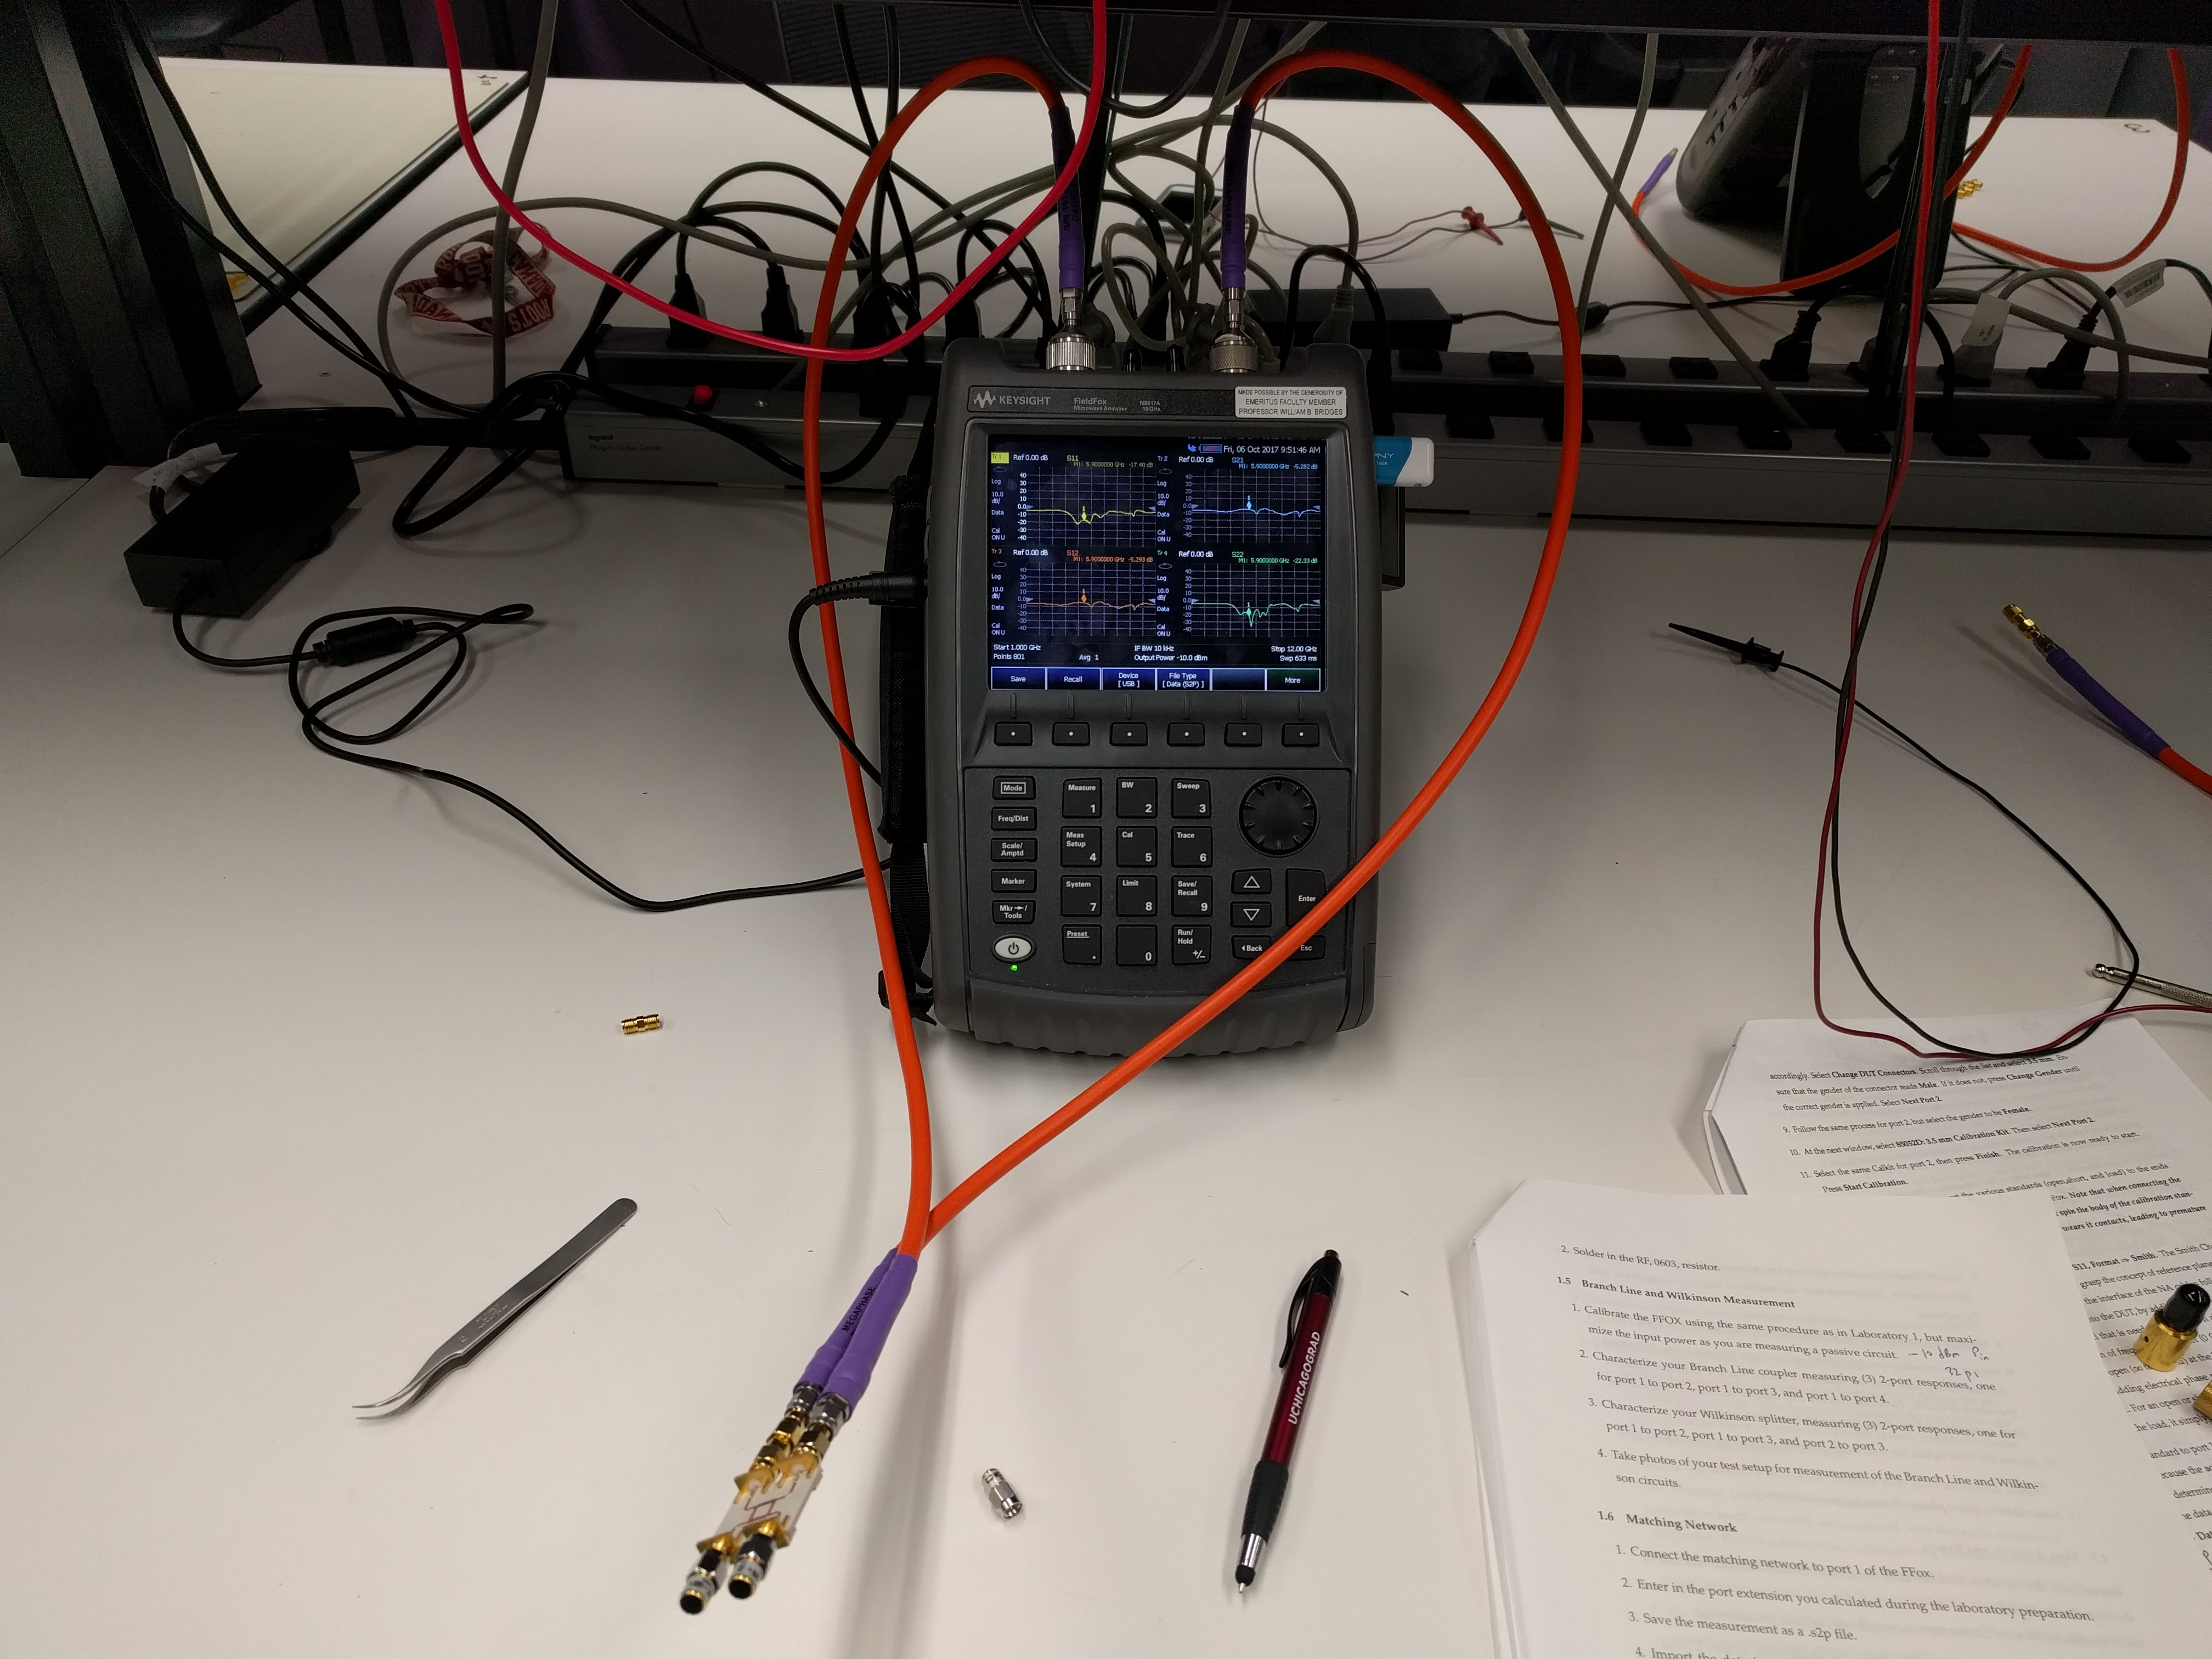
\includegraphics[scale=0.05]{BranchImg.jpg}
    \caption{Measurement Setup for the Branch Line Coupler}
    \label{fig:branchimg}
\end{figure}

\begin{figure}[!htbp]
    \centering
    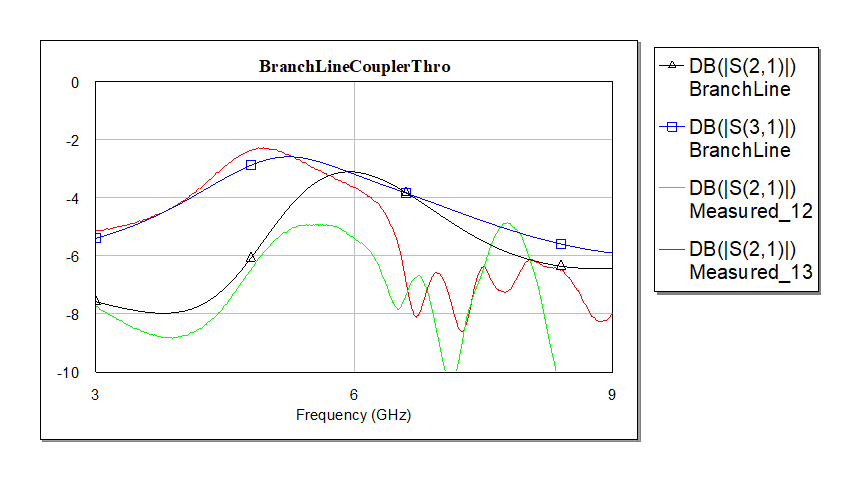
\includegraphics[scale=0.4]{BranchThro.png}
    \caption{Simulated vs. Measured through and coupled response of the Branch Line Circuit. }
    \label{fig:branchthro}
\end{figure}

\begin{figure}[!htbp]
    \centering
    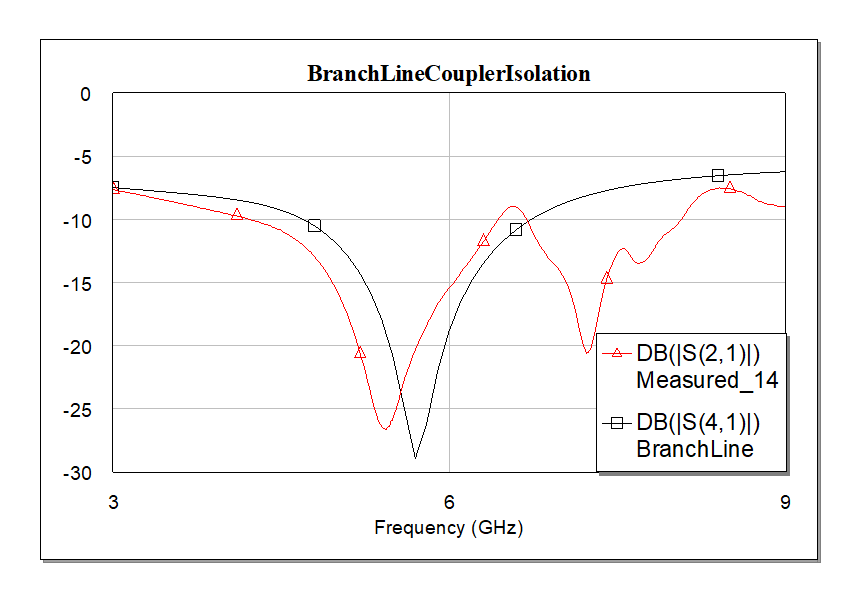
\includegraphics[scale=0.4]{BranchIsolation.png}
    \caption{A comparison between the simulated and measured isolation performance of the Branch Line Circuit.}
    \label{fig:branchiso}
\end{figure}


\begin{figure}[!htbp]
    \centering
    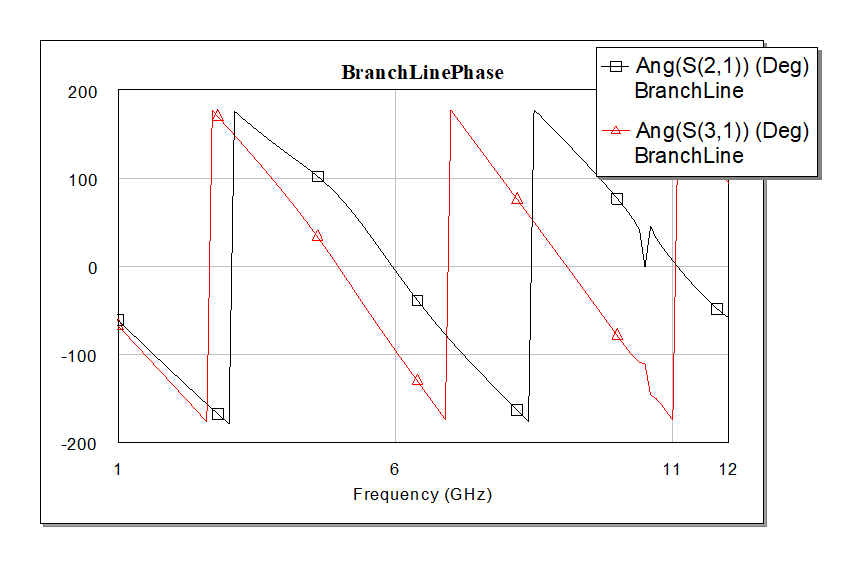
\includegraphics[scale=0.4]{BranchPhase.png}
    \caption{The simulated phase relationship between the two output ports as a function of frequency.}
    \label{fig:branchphase}
\end{figure}

One key difference between the simulation and measured response is the shift in the isolation resonance dip to lower frequencies. This meant that a better match was achieved at lower than design frequency. To match the measured response, I tuned the widths of the transmission lines (thus adjusting their characteristic impedances) as well as their lengths. $S_{31}$ was matched from 1-6.2 GHz \ref{fig:coupmatch} by varying both the line widths and the transmission line lengths. Above 6.2 GHz, a resonant dip in the transmission prevented a better match from being achieved. The characteristic impedance was changed to 50.45 $\Omega$ at a width of 46 mils and the length of the $Z_0$ transmission line adjusted to 163 mil which is about 0.87 of the previous value. $Z_1$ was tuned to $39.18 \Omega$ at a width of 75.5 mils while the length of the transmission line did not change significantly. With this parameters, $S_{21}$ and $S_{14}$ were also reasonably well matched as shown in figures \ref{fig:isolationmatch}, \ref{fig:thromatch}. From the simulations, we can conclude that the physical circuit had slightly shorter branch transmission lines that were wider than had been calculated. I also noted that the phase relationship at the output ports did not change much if at all after the lengths and widths were adjusted.

\begin{figure}[!htbp]
    \centering
    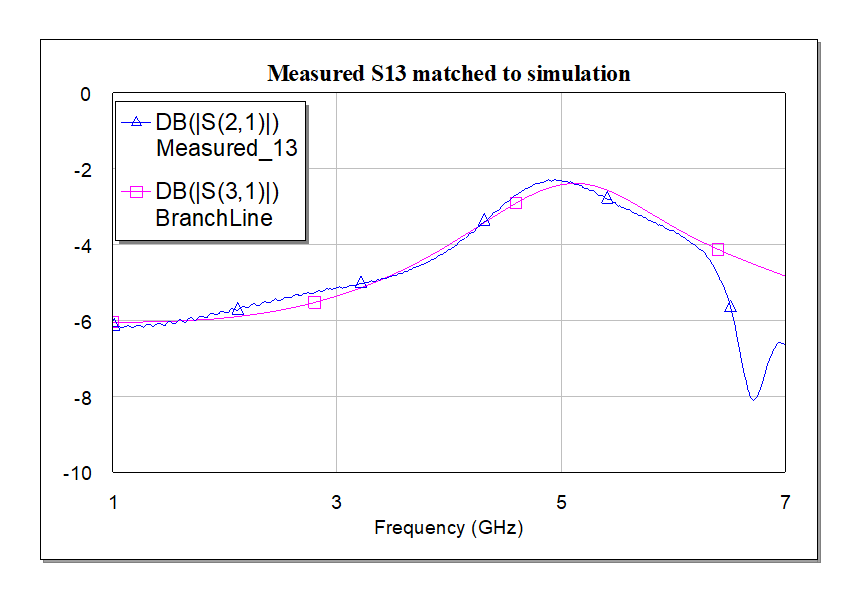
\includegraphics[scale=0.4]{CoupledMatch.png}
    \caption{The measured $S_{31}$ response matched by simulation. A good match was obtained up to about 6.2 GHz. }
    \label{fig:coupmatch}
\end{figure}

\begin{figure}[!htbp]
    \centering
    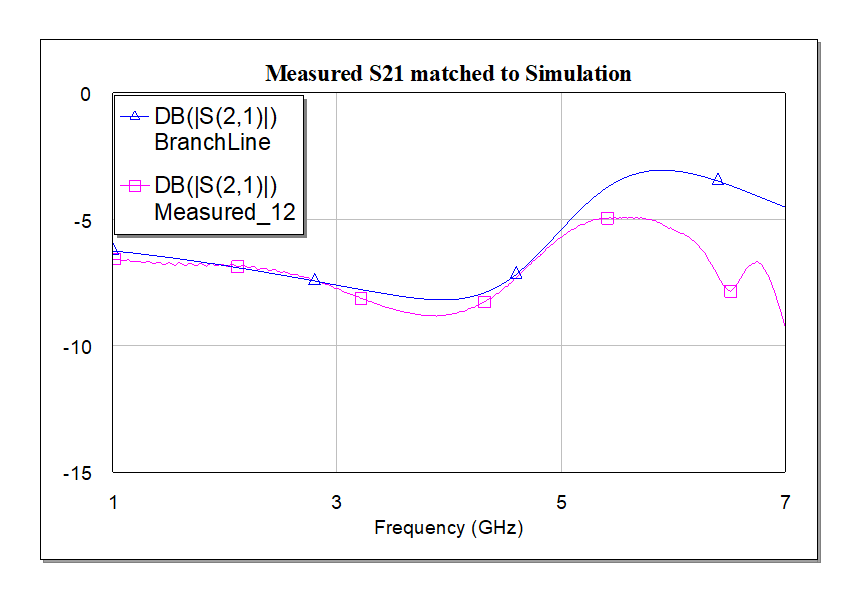
\includegraphics[scale=0.4]{ThroMatch.png}
    \caption{The measured $S_{21}$ response matched by simulation. At higher frequencies the measured response drops well below the simulated levels. }
    \label{fig:thromatch}
\end{figure}

\begin{figure}[!htbp]
    \centering
    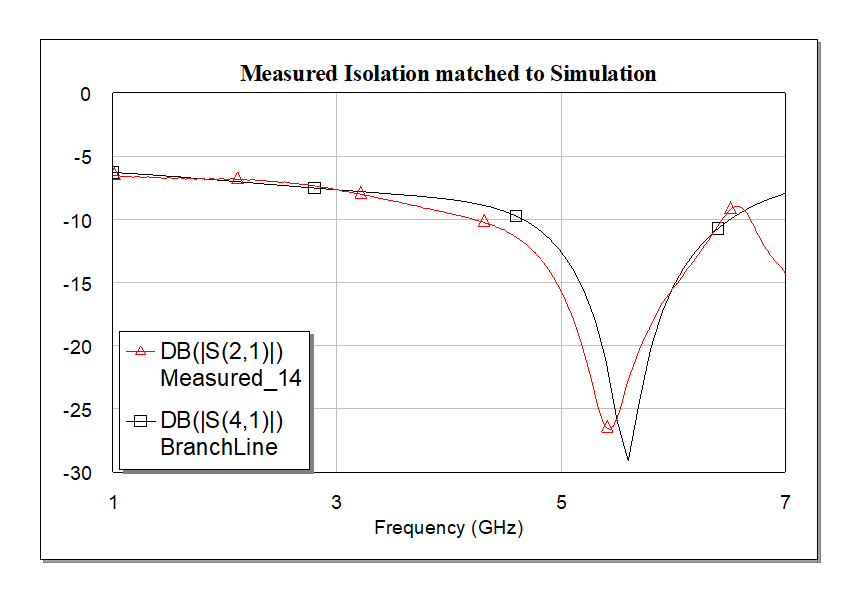
\includegraphics[scale=0.4]{IsolationMatch.png}
    \caption{The measured isolation ($S_{41}$) response matched by simulation. The measured resonant peak is shifted to slightly lower frequencies. }
    \label{fig:isolationmatch}
\end{figure}


Figure \ref{fig:thromatch} shows an additional resonance at 6.8 GHz in the measured through response of the circuit. This resonant feature may be responsible for the decreased performance of the circuit. A possible source of such resonances would be parasitic inductive and capacitive connections in the solder joints connecting the SMA launches and the circuit. To model this, I added a shunt inductor and a series capacitor to all ports of the circuit and tuned it to try and match the measured response. However, I could not find a suitable choice of the inductance and capacitance that would match the resonant wiggles seen in the S parameters. In addition, we considered detuning by the SMA launchers and circuit tolerances and used the LC network in the place of changes to the transmission line dimensions to try and match the measured and simulated S parameters. However, the choices of L and C were not well constrained and there were many combinations that I could choose that would qualitatively give me a good match between the two graphs. One such suitable choice for the shunt inductance was 7.8 nH with 4.1 pF of series capacitance. For the shunt L, series C network, a better match was obtained for larger values of L and C as the values given show. 

Lastly, we considered the dielectric substrate itself as a possible source of the mismatch. The substrate material datasheet lists 2 different values; 10.2 and 10.8 for the dielectric constant as measured by different techniques. Since the circuit was simulated using a dielectric constant of 10.2, a differing dielectric constant could be responsible. Instead of tuning the dielectric constant of the substrate, we adjusted the thickness of the substrate which similarly achieves the desired goal of tuning the effective dielectric constant of the microstrip. The best match I could obtain in this way was at about 46 mil substrate thickness. However, the quality and frequency range of the match were much poorer than the results obtained simply by adjusting the transmission line dimensions.



\FloatBarrier

\section*{Wilkinson Power Divider}\label{sec:Wilkinson}
\subsection{Design}
The Wilkinson Power Divider is a passive transmission line network that divides the input power equally between two output ports. By the three criteria discussed in the introductory section; the Wilkinson power divider is matched and reciprocal and thus necessarily lossy. Using this information, we can already deduce a lot about the scattering matrix of the Wilkinson Power Divider. First, the matching condition implies that all the reflection coefficients will be zero. As a result, we can set $S_{11} = S_{22} = S_{33} = 0$. The reciprocal condition can be written as $S_{12} = S_{21}, S_{13} = S_{31}, S_{23} = S_{32}$. Since the power is divided equally between the two output ports, we can conclude that $S_{21} = S_{31} = e^{j \phi}/\sqrt{2} $, where $\phi$ is the phase between the input and output signal waves. Unlike a Branch Line Coupler, the two outputs are in phase. Strong isolation between the two output ports sets $S_{23} = 0$We can thus write the scattering matrix as 

\begin{equation}
S = \frac{e^{j \phi}}{\sqrt{2}}
\begin{pmatrix}
    0 & 1 & 1 \\
    1 & 0 & 0 \\
    1 & 0 & 0 \\
\end{pmatrix}
\end{equation}

The phase $\phi$ can then be determined by analyzing the network. In addition, we need to determine the characteristic impedance $Z_c$ and the value of the resistor r. To do so, we will use the method of even and odd modes to take full advantage of the circuit's high symmetry. We will assume that a voltage $+2 V_s$ is applied to port 2 (since the network is reciprocal) through a matched resistor whose resistance equals the characteristic impedance of the line $Z_0 = 50 \Omega$. We will also terminate port 1 with a matched 50 $\Omega$ resistor R. Port 1 can be divided into 2 circuits by considering the resistor R as 2 parallel resistors connected at port 1, each with resistance 2 R. The resistor r can be divided into 2 resistors in series, each with resistance r/2. We can make the symmetry even more explicit by adding 2 voltage sources at port 3; $+V_s$ and $-V_s$ to deliver a net 0 voltage through a matched 50 $\Omega$ resistor. 

For the even mode, we consider the two +V sources at port 2 and 3. Now, in the midplane of the circuit, there is no potential drop across the connecting line and therefore no current flows through it. We can thus divide the circuit across the symmetry line replacing the cut ends with open circuit terminations and only consider the top circuit. A schematic of the even mode circuit is shown in figure \ref{fig:evenmode}. Since the resistor r/2 is terminated by an open circuit connection, it plays no role in the even mode circuit. Only the transmission line matters. The quarter wave line acts as an impedance transformer on the load impedance ($Z_L =2 Z_0$) at port 1, giving the input impedance at port 1 $Z_{in} = Z_c^2/(2 Z_0)$. Since the Wilkinson is matched, the input impedance as seen from port 2 must equal $Z_0$. Therefore $Z_c = \sqrt{2 Z_0^2} = \sqrt{2} Z_0 = 70.71 \Omega$ for the matched load. Now at port 2, $V_2^e = + V_s/2 = V_3^e$ since there is a voltage divider. We need to use the transmission line equations to find the voltage at port 1. The voltage in a transmission line of length l (origin at input) is given by the equation

\begin{figure}[!htbp]
    \centering
    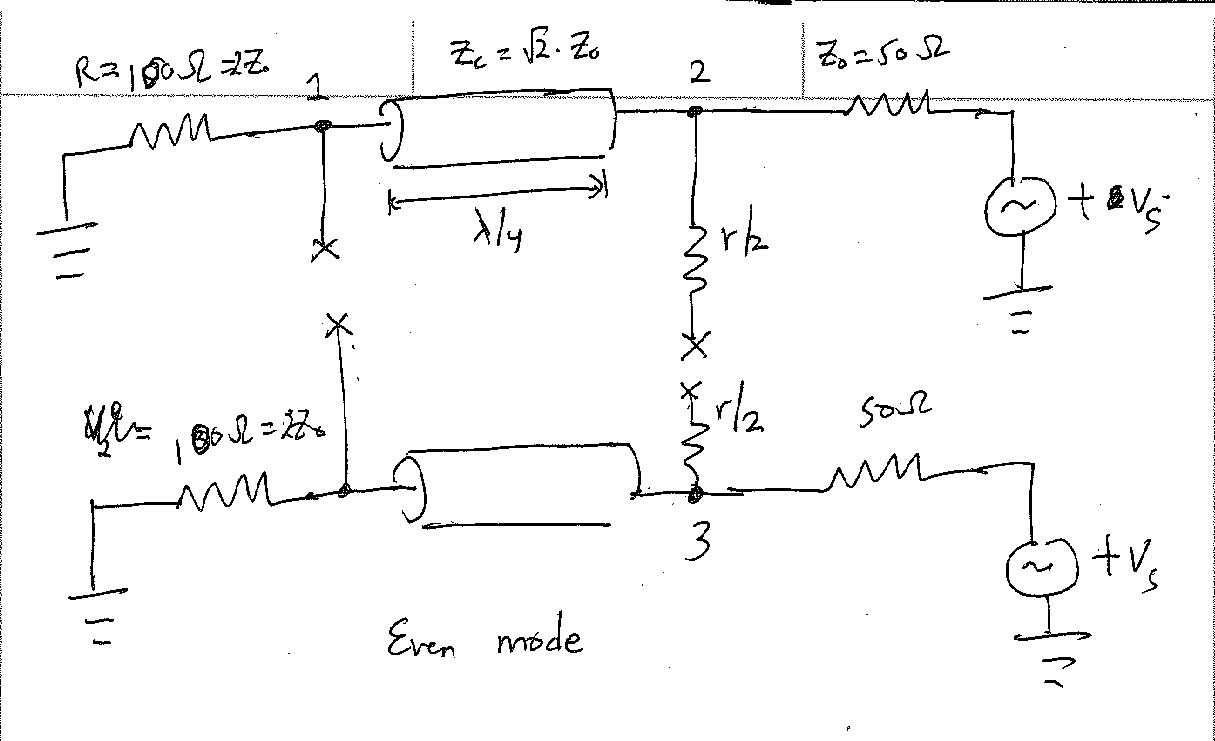
\includegraphics[scale=0.2]{EvenMode.png}
    \caption{Even Mode circuit for the Wilkinson power divider. }
    \label{fig:evenmode}
\end{figure}


\begin{equation}
    V(l) = V^+ \left(e^{j \beta l} + \Gamma e^{-j \beta l}\right)
\end{equation}

Thus $V_2^e = V^+ \left(1 + \Gamma \right)$ and $\Gamma = (\sqrt{2} - 1)/(\sqrt{2} + 1)$. $V^+$ is the incoming voltage wave. At port 1, $V_1^e = j V^+ \left(1 - \Gamma \right) $.Using the expression for $V_2^e$ to substitute for the incoming voltage wave gives

\begin{align*}
    V_1^e &= \left(\frac{j V_s}{2}\right) \left(\frac{1 - \Gamma}{1 + \Gamma}\right) \\
    &= \left(\frac{j V_s}{2 \sqrt{2}}\right)
\end{align*}

For the odd mode circuit, port 2 has a voltage $+V_s$ while port 3, $-V_s$. In this case, at the symmetry line, the voltage must go to zero at the midplane and we have a virtual ground plane. We can similarly divide the circuit across the symmetry line replacing the terminations with ground connections as shown in figure \ref{fig:oddmode}. In this case, the short circuits to ground at port 1 isolates the load network from the input. In addition, as seen from port 2, the quarter wave line is an open circuit since it is shorted to ground. Thus we only have the resistance $Z_0$ in series with the resistance r/2. In order to satisfy the matching criterion then, r = 100 $\Omega$. Again, $V_2^o = V_s/2 = - V_3^o$. $V_1^o = 0$ since the port is grounded. Combining the even and odd mode values gives

\begin{figure}[!htbp]
    \centering
    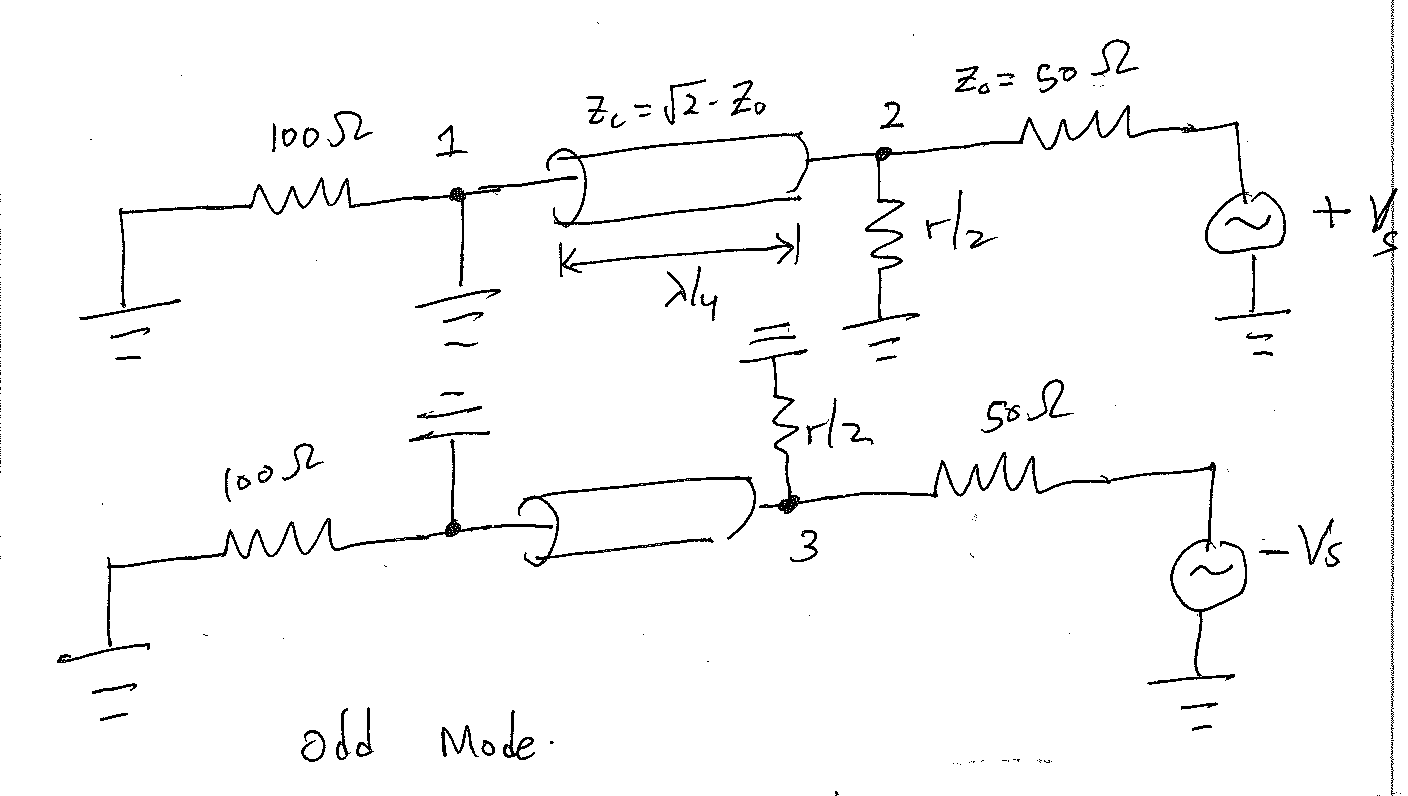
\includegraphics[scale=0.2]{OddMode.png}
    \caption{Odd Mode circuit for the Wilkinson power divider. }
    \label{fig:oddmode}
\end{figure}

\begin{align*}
    V_2 &= V_2^e + V_2^o = V_s \\
    V_1 &= V_1^e + V_1^o = \frac{j V_s}{2 \sqrt{2}} \\
    V_3 &= V_3^e - V_3^o = 0
\end{align*}

Now that we've determined the voltages at each of the ports, we need to find all the terms of the S matrix. At each terminal we have the sum of the incoming and outgoing signal waves. However, since ports 1 and 3 have matched loads at their terminals, they have no reflections at the terminals. Port 2 has also been connected to the source through a resistor equal to the characteristic impedance of the line. Therefore we conclude the S parameters are

\begin{align*}
    S_{12} &= S_{21} = \frac{V_1}{V_2} = \frac{j V_s}{2 \sqrt{2}} \frac{2}{V_s} = \frac{-j}{\sqrt{2}} \\ 
    S_{32} &= S_{23} = \frac{V_1}{V_2} = 0 \\
    S_{22} &= 0 \\
    S_{33} &= 0 \textrm{(since port 2 and 3 are identical)}\\ 
    S_{13} &= S_{31} = \frac{-j}{\sqrt{2}} \textrm{(since port 2 and 3 are identical)}\\ 
\end{align*}
We had already concluded that $S_{11} = 0$ and thus we've showed that $\phi = \pi$.

\begin{equation}
S = \frac{-j}{\sqrt{2}}
\begin{pmatrix}
    0 & 1 & 1 \\
    1 & 0 & 0 \\
    1 & 0 & 0 \\
\end{pmatrix}
\end{equation}

Based on the calculated $Z_c = 70.71 \Omega$ and $Z_0 = 50 \Omega$, we designed transmission lines with these characteristics in Microwave Office. The transmission lines microstrip just as in the Branch Line case. The widths of the microstrip lines for the desired characteristic impedances were calculated using the TXLine program in Microwave Office and are summarized in table \ref{tab:wilkinson} summarizes the dimensions of the Wilkinson divider after the circuit was optimized for power transmission at 5.9 GHz. 

\begin{table}
\centering
\begin{tabular}{l | c | c}
    \hline
    Z [$\Omega$] & W [mils] & $\lambda/4$ [mils] \\
    \hline
    50  & 46.0 & 187.0 \\
    70.71 & 16.0 & 225.0 \\
    \hline
\end{tabular}
\caption{Parameters of the transmission lines used in the Wilkinson divider. All dimensions have been rounded to the nearest half mil and the values reported are the optimized values to center the circuit response at 5.9 GHz. }
\label{tab:wilkinson}

\end{table}

Using the circuit design, we made a layout and routed the input and output lines to fit the 1x1 inch circuit size. The spacing between the input and output traces was set to about 500 mils for ease of mounting the SMA connectors.

\subsection{Lab Testing and Analysis}

The lab measurements closely parallelled the Branch Line Measurements. We measured 3 2-port responses of the branch line coupler; $S_{21}, S_{31}$ and $S_{41}$. The results in comparison to the simulated circuit response are shown in figure \ref{fig:wilkinsonmag} and the experimental setup is shown in figure \ref{fig:wilkinsonimg}


\begin{figure}[!htbp]
    \centering
    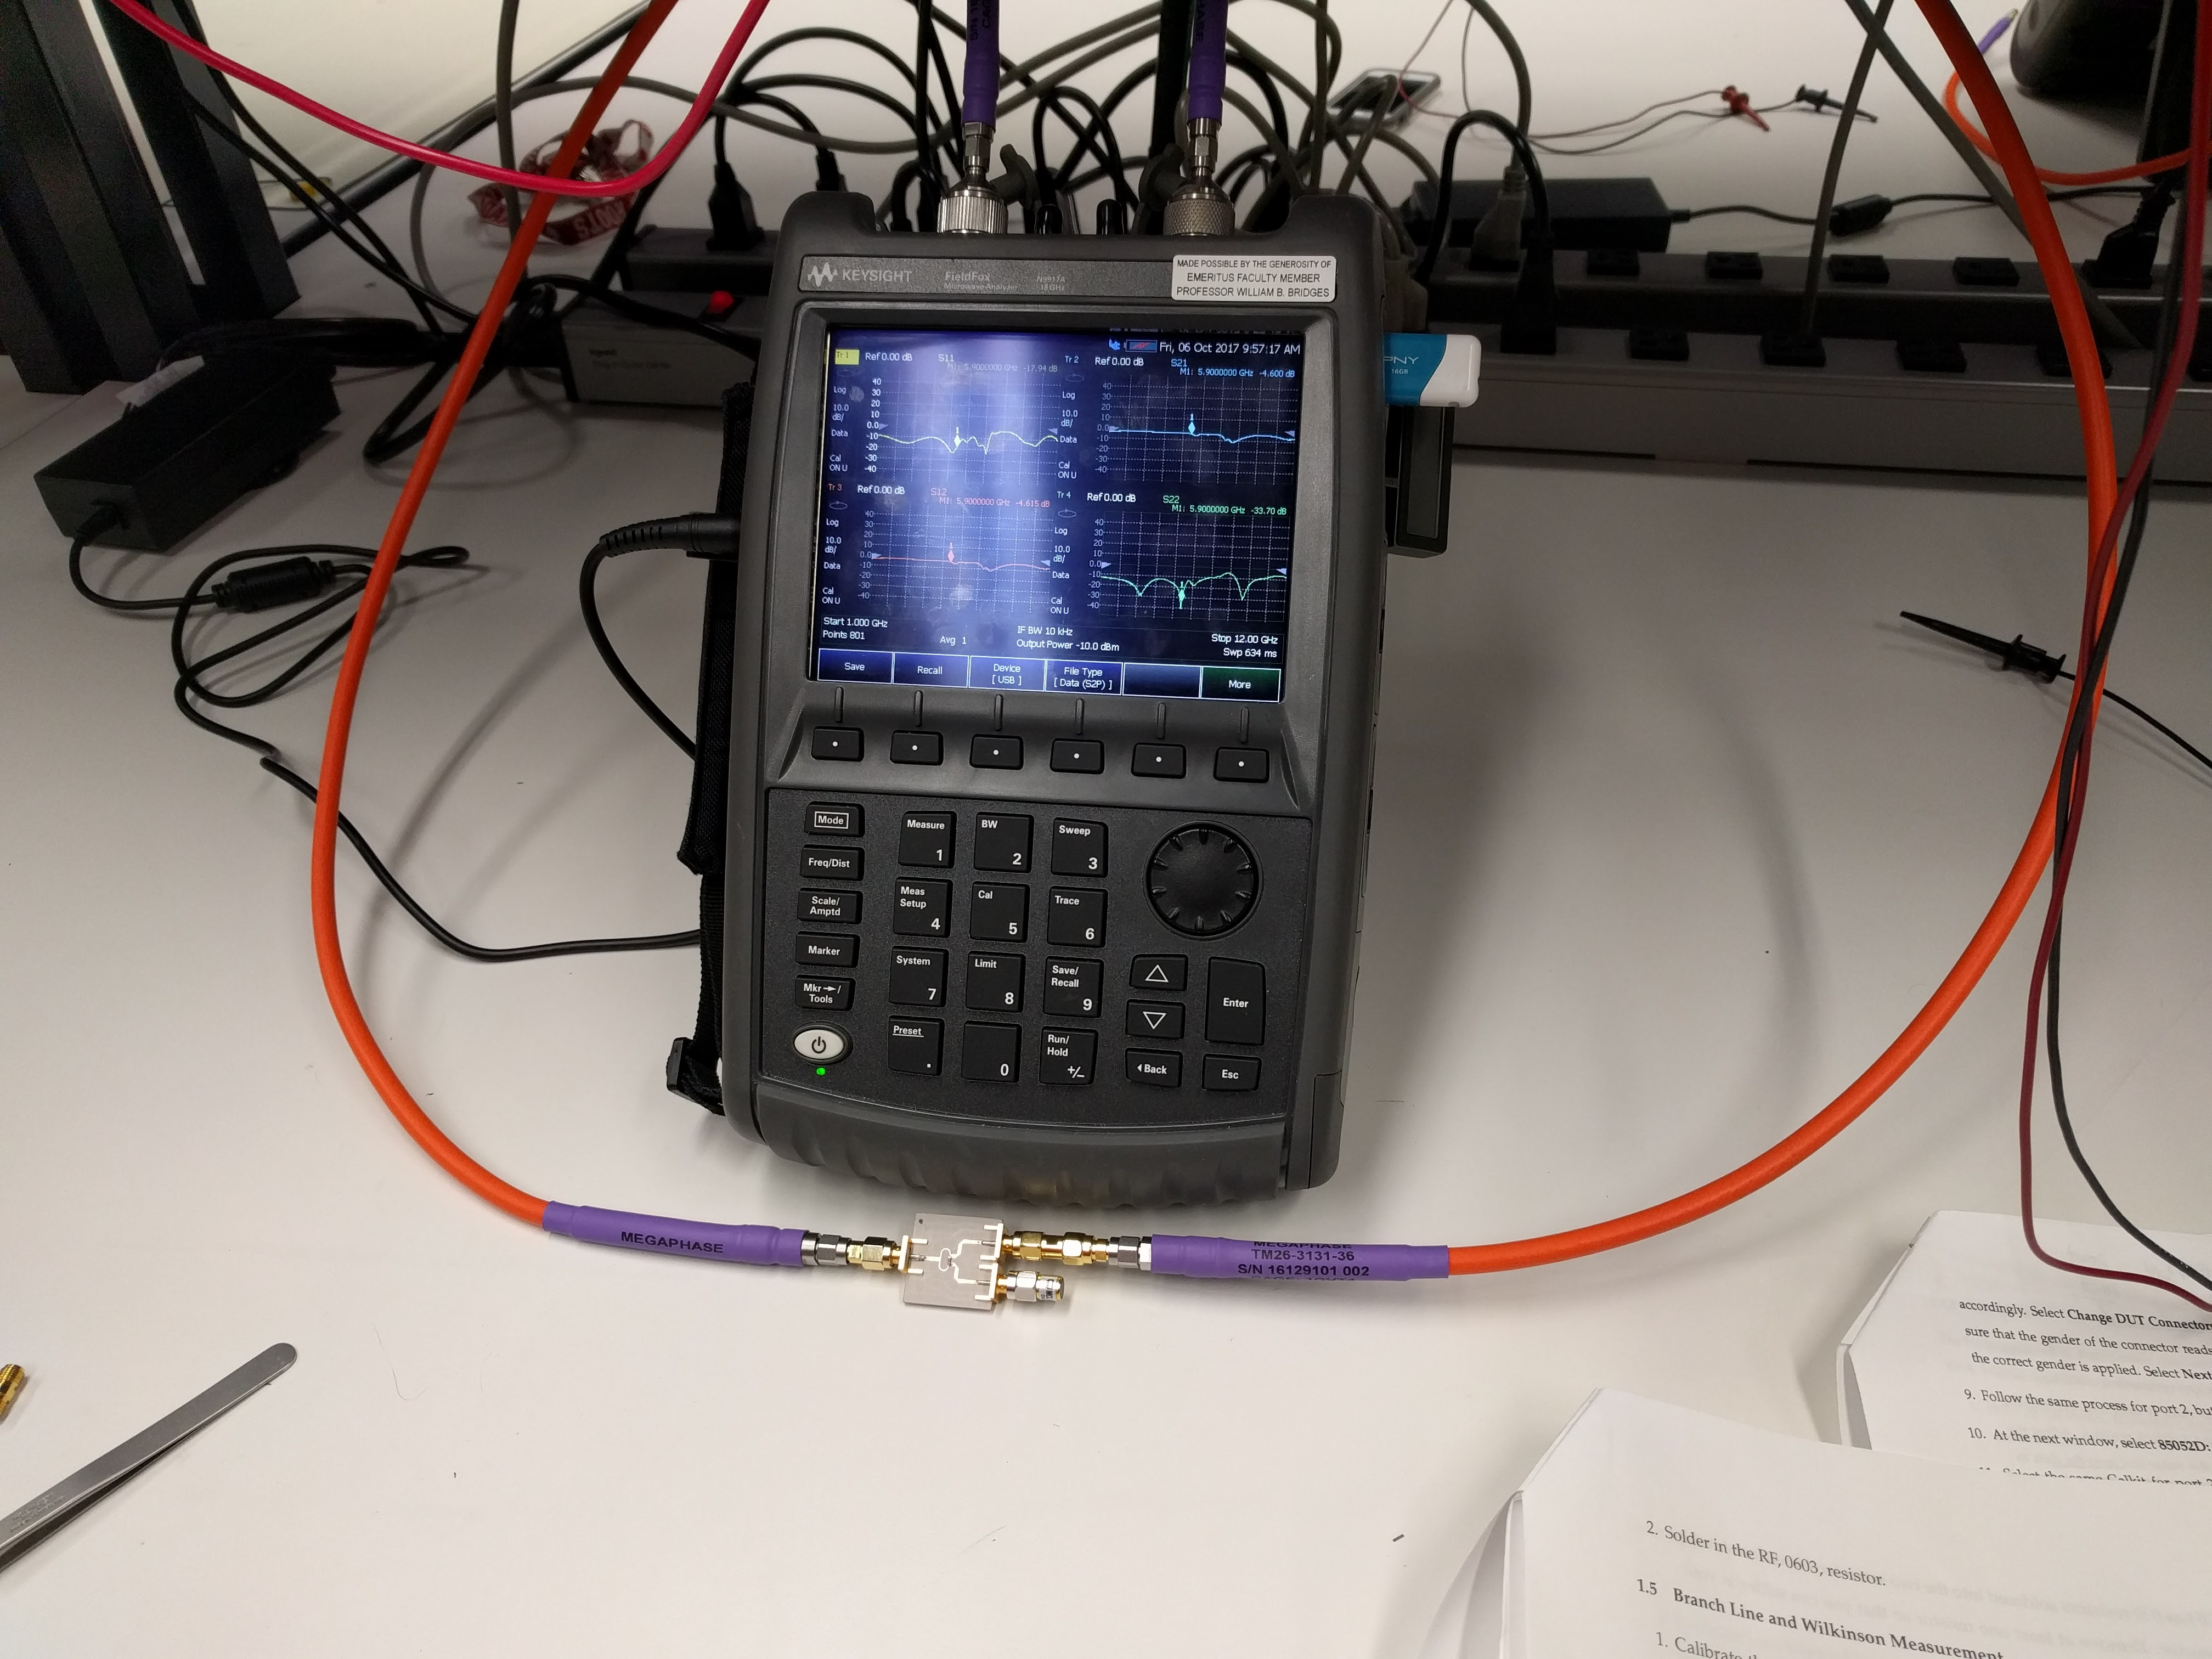
\includegraphics[scale=0.05]{WilkinsonImg.jpg}
    \caption{Measurement Setup for the Wilkinson Power Divider.}
    \label{fig:wilkinsonimg}
\end{figure}


\begin{figure}[!htbp]
    \centering
    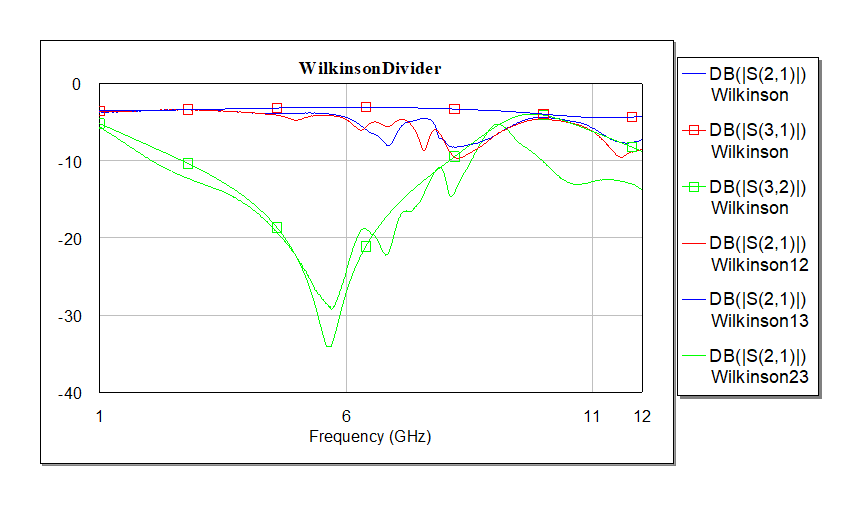
\includegraphics[scale=0.4]{WilkinsonCircuit.png}
    \caption{A comparison between the simulated and measured performance of the Wilkinson Power Divider.}
    \label{fig:wilkinsonmag}
\end{figure}

From figure \ref{fig:wilkinsonmag}, the simulated and measured isolation performance between ports 2 and 3. However, ports 2 and 3 significantly underperform. Above about 3.0 GHz, $S_{21}, S_{31}$ begin to slow dip down below the -3 dB level. Quite similarly to the branch line case, tuning the transmission line widths and length gives a much improved match with the measured response. $S_{31}$ is well matched between 2.8 and 5.4 GHz as shown in figure \ref{fig:wilkcoup}. Above this, the resonant peak at 6.8 GHz decimates the circuits performance. The isolation is shown in figure \ref{fig:wilkiso} as a comparison. For $S_{21}$, shown in figure \ref{fig:wilkthro}, the match is not nearly as good. Interestingly, $S_{21}$ shows additional resonant dips at 5.0 GHz and 6.3 GHz. Since these peaks do not show up in $S_{31}$ they may be due to effects confined to port 2 only and not inherent to the entire circuit design. A likely cause may be due to poor solder connections between the port 2 SMA launcher and the microstrip line. Parasitics at the port may modify the S parameter being read out by the VNA. The parameters that best match the measured response are for $Z_0 = 59.3 \Omega$ at a line width of 31.6 mils. In addition the $Z_c$ line is adjusted to a width of 24.6 mils and a length 219 mils. This gives a much lower $Z_c = 65.2 \Omega$ at about 1.1 times the quarter wavelength length. The most surprising bit is the much higher $Z_0$. It doesn't match the shift in $Z_0$ from the Branch Line circuit and thus isn't a result of the fabrication tolerances. Curiously though, the resonant feature at 6.8 GHz appears in both the Branch Line and Wilkinson circuits. Since they were fabricated on the same substrate, it could likely be a result of some common fabrication tolerances or common weaknesses in the similar modeling techniques used for both circuits. Microwave Office doesn't solve for the full Maxwell's equations and thus may introduce some uncertainty.


\begin{figure}[!htbp]
    \centering
    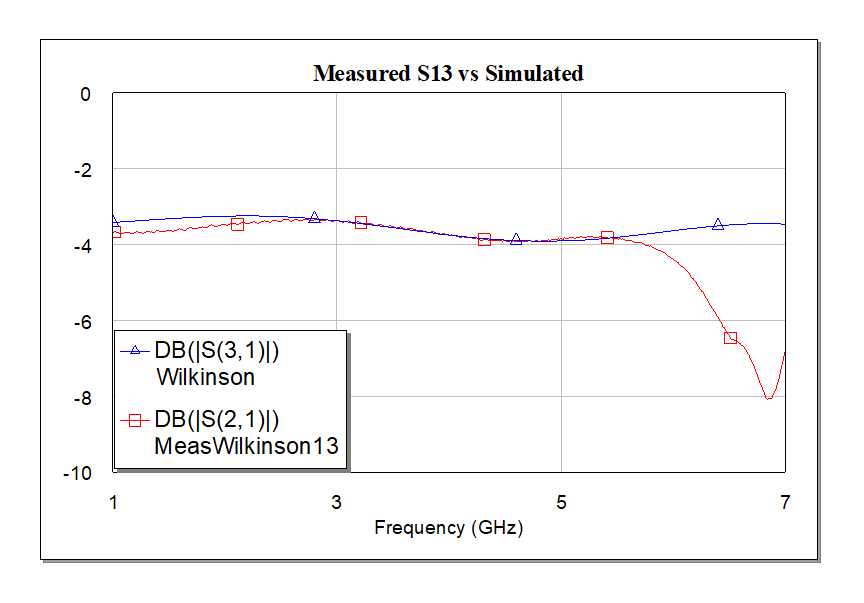
\includegraphics[scale=0.4]{WilkinsonCoupled.png}
    \caption{The measured $S_{31}$ response matched by simulation. }
    \label{fig:wilkcoup}
\end{figure}

\begin{figure}[!htbp]
    \centering
    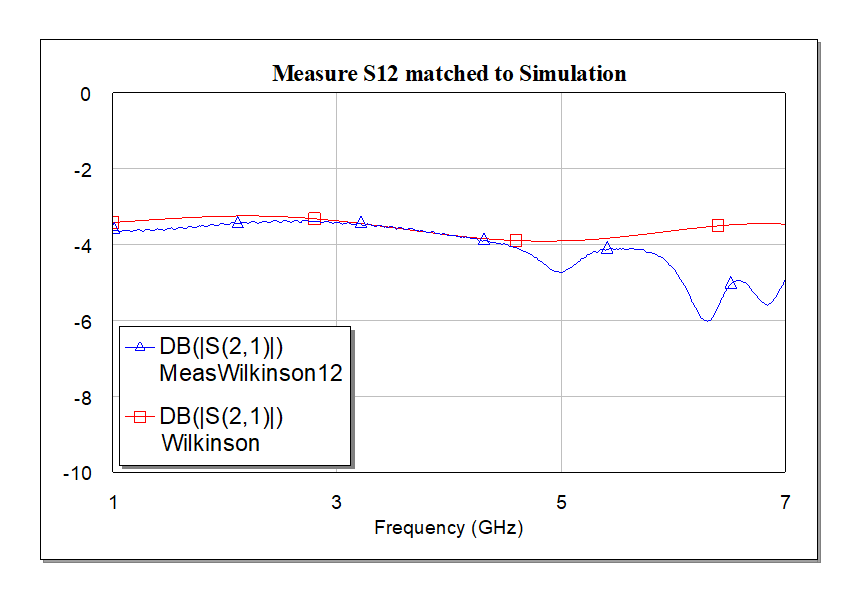
\includegraphics[scale=0.4]{WilkinsonThro.png}
    \caption{The measured $S_{21}$ response matched by simulation. Note the series of resonant dips between 5 and 7 GHz. }
    \label{fig:wilkthro}
\end{figure}

\begin{figure}[!htbp]
    \centering
    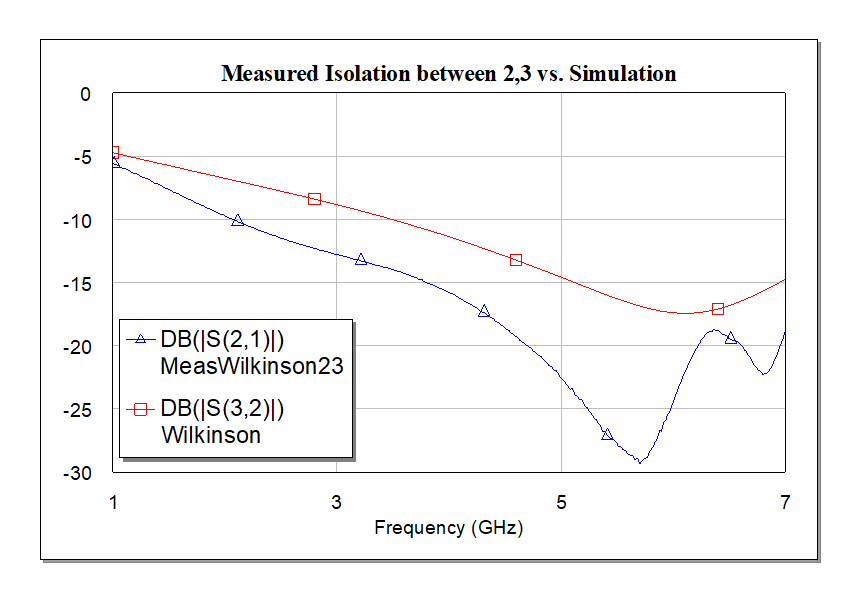
\includegraphics[scale=0.4]{WilkinsonIso.png}
    \caption{The measured isolation ($S_{41}$) response matched by simulation. The measured resonant peak frequency matches well with the simulated. }
    \label{fig:wilkiso}
\end{figure}

\FloatBarrier

\section*{Impedance Matching}\label{sec:ImpedanceMatching}

We designed a lumped element matching network for an already populated RC network on a circuit board as shown in figure \ref{fig:RCimg}. To do so, we first measured $S_{11}$ for the RC circuit to obtain its input impedance as a function of frequency to match it at 4 GHz. In order to make the measurement of the RC circuit S parameter, it was necessary for us to adjust the reference plane to account for the electrical delay due to the SMA connector and microstrip section that connected the RC circuit to the NA. The time delay $\tau$ at the frequency $f$ can be calculated from the electrical delay $\phi$ given as a phase angle (as is done in TXLine) using the equation $\tau = \frac{\phi}{2 \pi f}$. The coaxial line of the SMA connector was 290 mil long with a 50 mil diameter inner conductor and a 168 mil diameter outer conductor. Teflon, which fills the coax line, has a dielectric constant of 2.1 giving an electrical length of 51.27 \textdegree. The microstrip section which was 430 mil long on 12 mil thick FR-4 (dielectric constant of 4.4) had an electrical length of 95.37 \textdegree for a 20 mil wide traces that was 1.7 mils thick. Using the time delay equation and the total electrical length obtained from TXLine, we obtained the total time delay of the circuit as 101.8 ps. This was the value used to move the reference plane of the VNA to the plane of the RC network.

The matching network was designed in MWO using a Smith Chart to achieve a match with a 50 $\Omega$ line at 4 GHz. The load impedance at 4 GHz was measured to be $Z = 17.91 - j 17.80 \Omega$. On the Smith Chart, a match is obtained by moving the impedance point along circles of constant resistance/conductance until the intersection with either the r=1 or the y=1 circle is reached. Clockwise motion along impedance circles adds series inductance while counterclockwise motion adds series capacitance. On admittance circles, clockwise motion adds shunt capacitance while counterclockwise motion adds shunt inductance. The designed matching network had the parameters series L = 1.66 nH and shunt C = 1.065 pF. However, in lab, we were only able to find L = 1.8 nH and C = 1.0 pF elements. Using these, we were only able to achieve the match showed in figures \ref{fig:RCmatched} and \ref{fig:RCsmith}. From the plots, it is clear that a much better match was achieved at about 3.67 GHz with 11 dB return loss. We modelled the inductor and capacitors as closed form elements. A more accurate match would have required the use of the S parameter files from the manufacturer for more accurate simulations. Even so, we were able to achieve $Z_{in} = 42.58 -j 1.999 \Omega $ using our matching network. We were able to suitably match the network, albeit at lower than design frequencies. For better match, we would have used the S parameter files for more agreement between simulation and data. For example, using the L\-05C1N5\_SER.s2p inductor in the simulation gives $Z_{in} = 40.60 - j 1.077 \Omega$, which is in much closer agreement to the measured value.


\begin{figure}[!htbp]
    \centering
    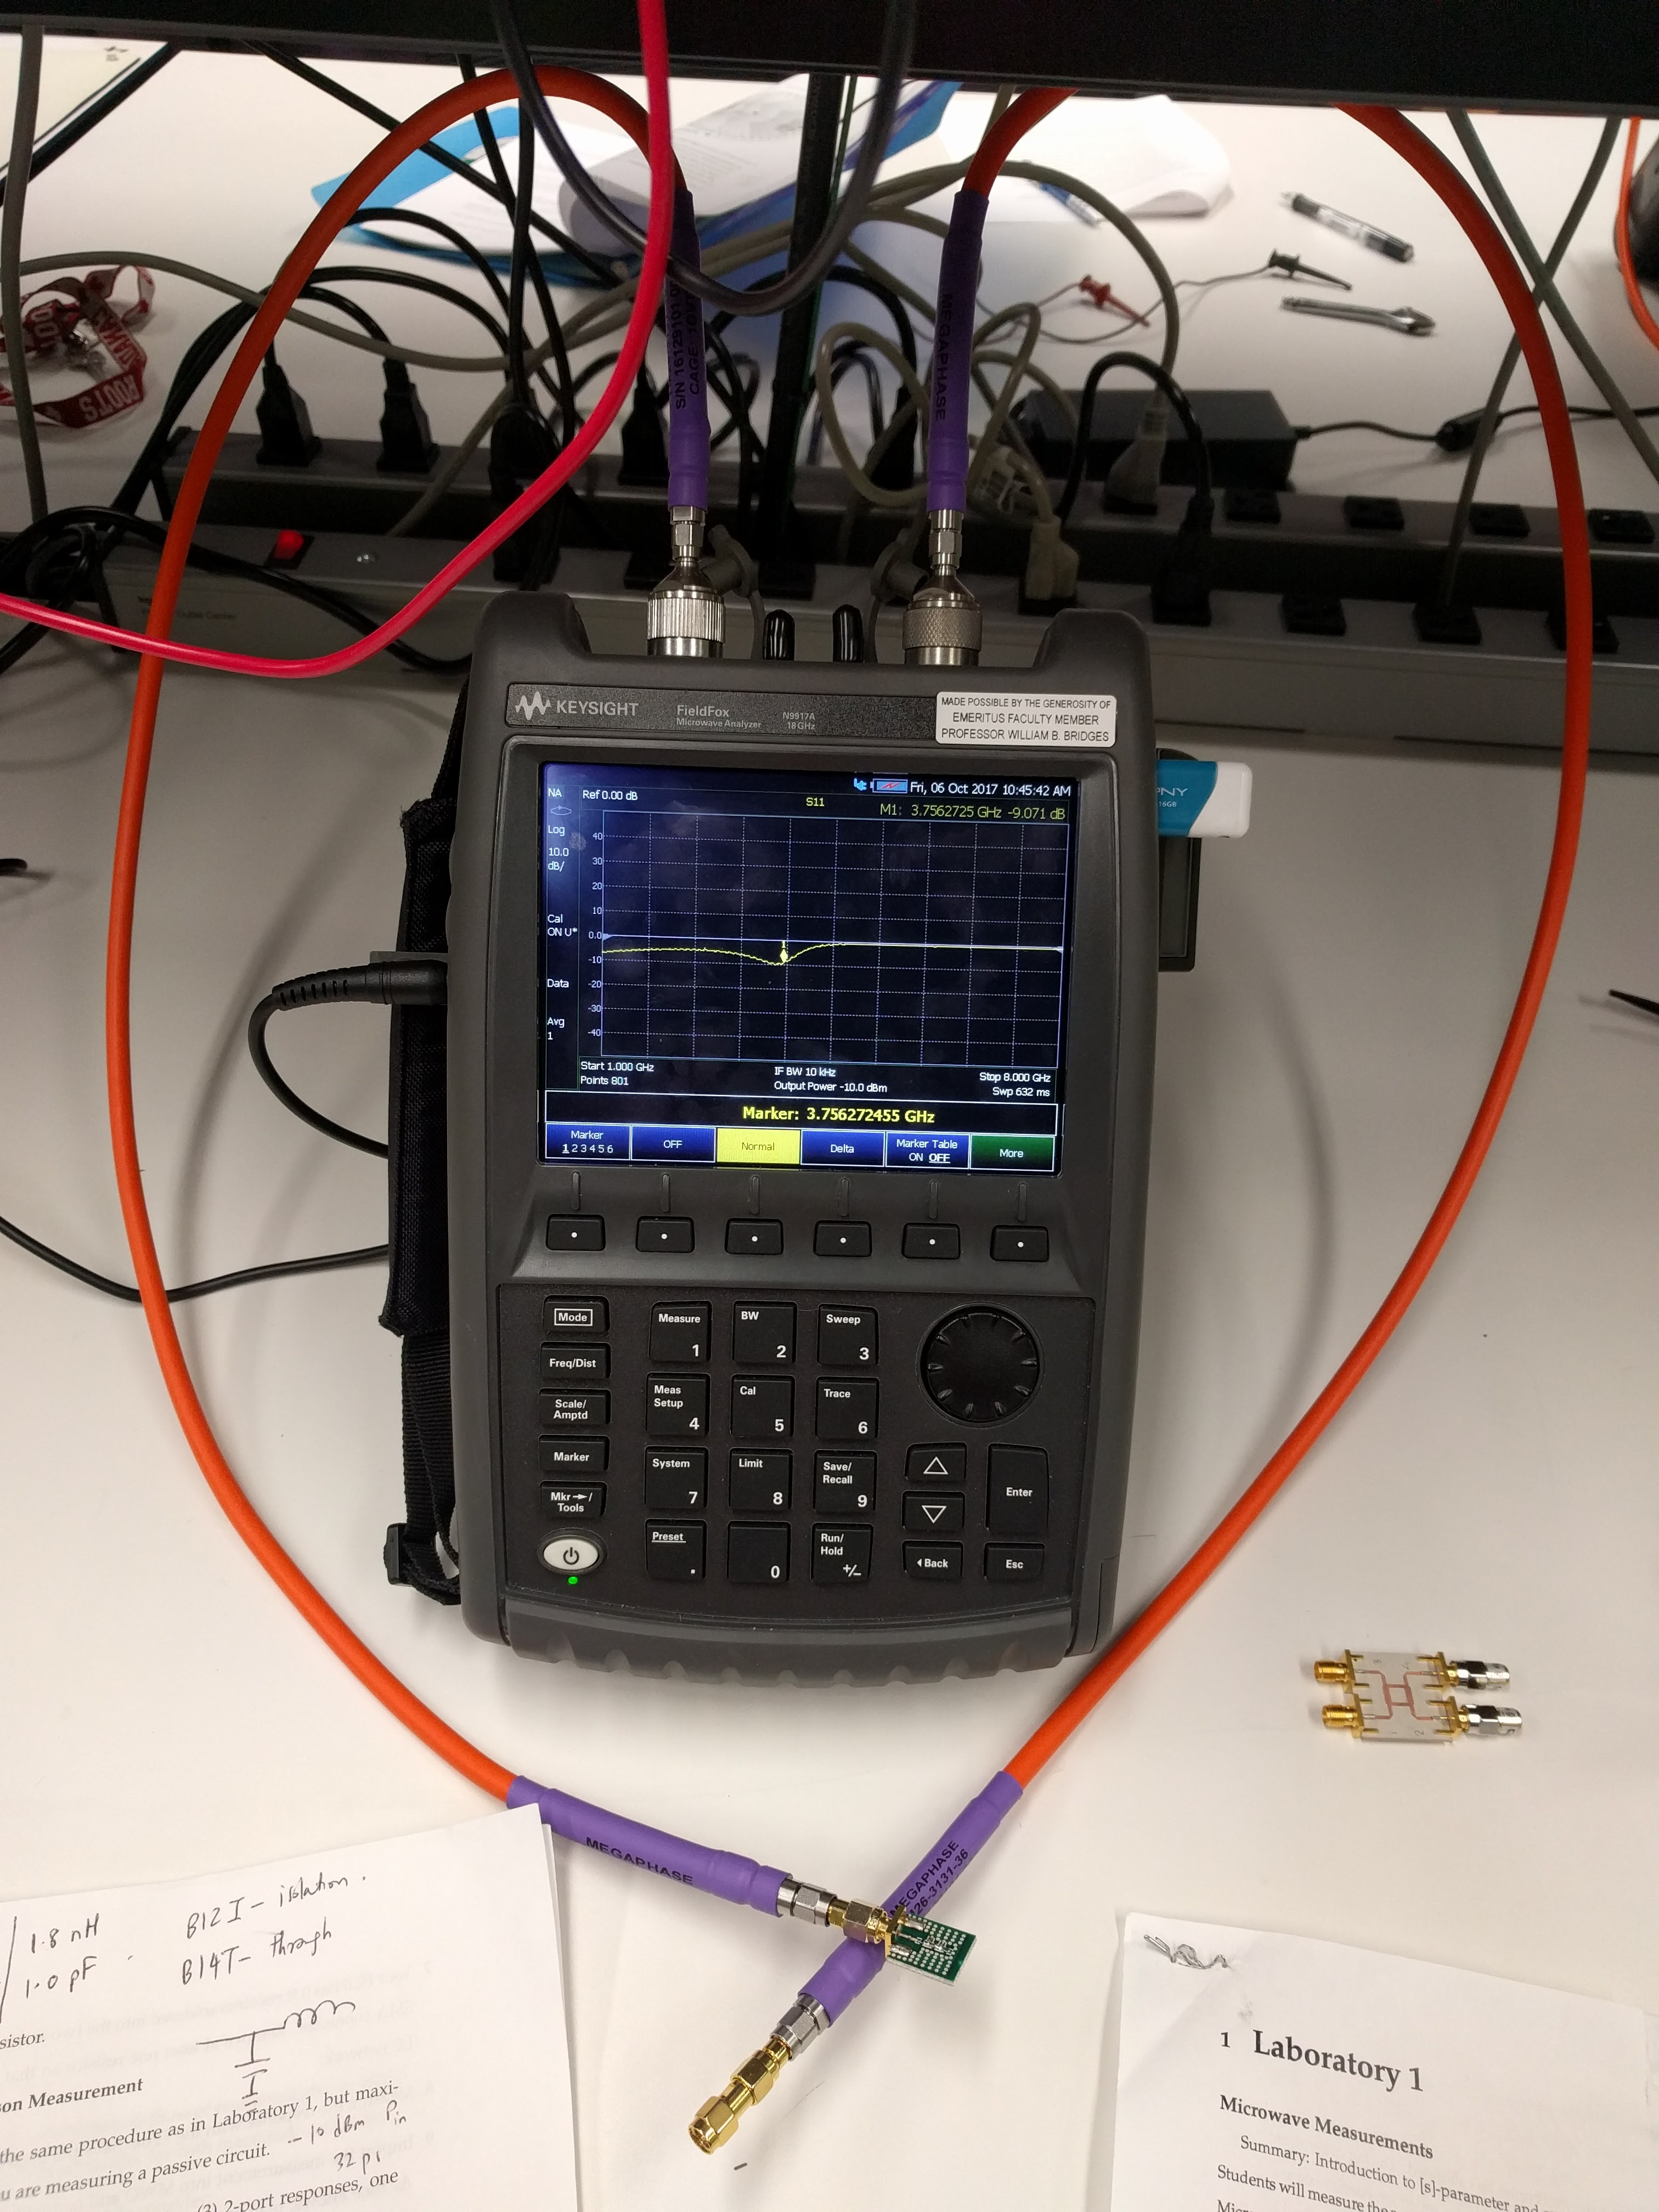
\includegraphics[scale=0.05]{RCImg.jpg}
    \caption{Measurement Setup for the RC Impedance Matching.}
    \label{fig:RCimg}
\end{figure}

\begin{figure}[!htbp]
    \centering
    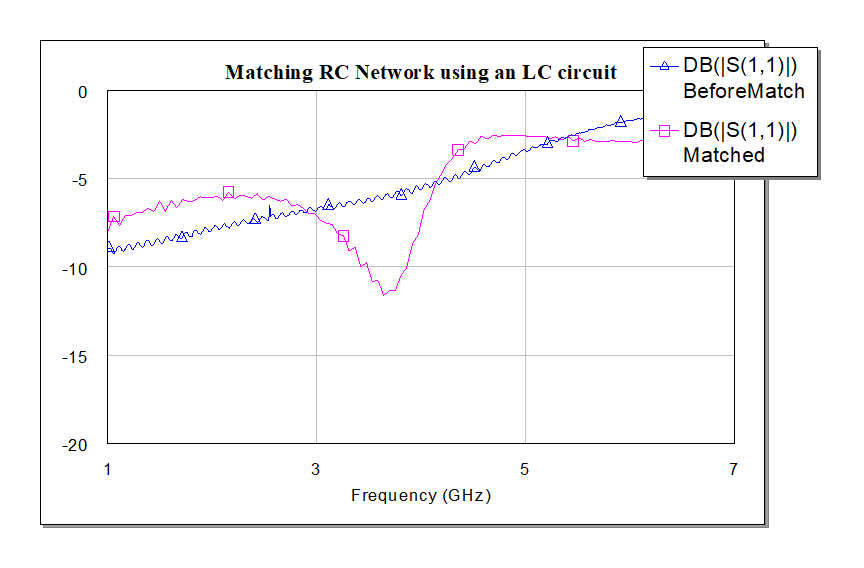
\includegraphics[scale=0.4]{RCMatched.png}
    \caption{Comparison of the RC Network before and after matching.}
    \label{fig:RCmatched}
\end{figure}

\begin{figure}[!htbp]
    \centering
    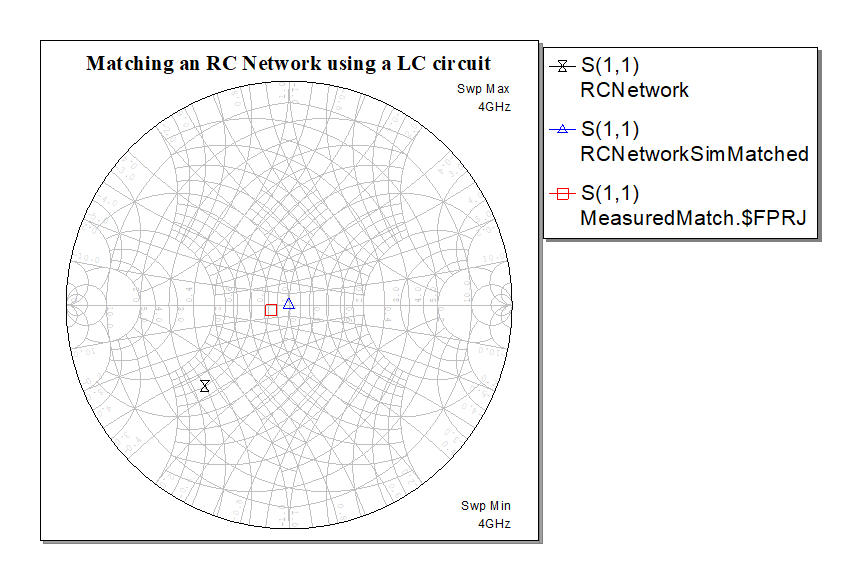
\includegraphics[scale=0.4]{RCSmith.png}
    \caption{Smith chart showing the point at 4 GHz simulated before and after the matching network was added. The actual measured value is also plotted.}
    \label{fig:RCsmith}
\end{figure}

\section*{Conclusions}
The biggest lesson I learned is that actual data is almost always going to differ from the simulations. As a circuit designer, I need to be aware of the limitations of my simulation tools as well as experimental technique in order to diagnose and correctly account for deviations from the model. Real circuit development would certainly require multiple iterations improving match, broadening bandwidth and meeting other such design specifications. I learned how to design power couplers and dividers to split power equally between two output ports. This also forced me to learn how to use even and odd mode analysis as a powerful technique for analyzing such circuits. In addition, I played around with creating matching circuits for arbitrary loads and developed an appreciation for the difficulty involved in achieving near perfect match at a specified frequency. This will certainly be useful in the next lab and many more future ones. The art of making good electrical solder joints was also a crucial practical aspect of this week's lab that I got to practice. 
\end{document}